\documentclass[aspectratio=169]{beamer}
\usetheme{Madrid}

% Pakete für die deutsche Sprache
\usepackage[T1]{fontenc}
\usepackage[utf8]{inputenc}
\usepackage[english]{babel}
\usecolortheme{seahorse}
\setbeamercolor{block title}{bg=blue!20,fg=black}

\usepackage{tikz}
\usepackage{graphicx}
\usepackage{listings}
\usepackage{hyperref}

% Stil für C-Code-Listings
\lstset{
  language=C,
  basicstyle=\ttfamily\footnotesize,
  keywordstyle=\color{blue},
  commentstyle=\color{green!50!black},
  stringstyle=\color{red},
  showstringspaces=false,
  breaklines=trü,
  frame=single,
  frame=none,
  captionpos=b,
  literate={ö}{{\"o}}1 {ä}{{\"a}}1 {ü}{{\"u}}1,
}

\title{Linux Driver Workshop}
\subtitle{An introduction to Linux Driver Development}
\author{Johannes Roith}
\date{16.08.2025}

\begin{document}

\begin{frame}
  \titlepage
\end{frame}

\begin{frame}{About me}
	\begin{itemize}
		\item Embedded Software Developer
		\item \href{https://www.youtube.com/@johannes4gnu_linux96}{Embedded Linux YouTube Channel}
		\item \href{https://gnu-linux.rocks}{\textcolor{blue}{My website}} with links to my GitHub, Mastadon, LinkedIn, \dots
		\item One driver of mine made it into the Linux Kernel
	\end{itemize}
\end{frame}

\begin{frame}{Agenda}
	\tableofcontents[sections={1-10}]
\end{frame}

\begin{frame}{Backup}
	\tableofcontents[sections={11-}]
\end{frame}

\section{The Linux Kernel}
\begin{frame}{The Linux Kernel}
	\begin{itemize}
		\item Kernel of an operating system: hardware abstraction layer
		\item Uniform interface (API Systemcalls) independent from PC architecture
		\item Tasks of the Linux-Kernels:
			\begin{itemize}
				\item Memory management
				\item Process management
				\item Multitasking
				\item Load balancing
				\item Access to hardware over drivers
			\end{itemize}
		\item Applications are using systemcalls (open, close, read, write, ioctl, \dots{}): they don't need knowledge about the underlying hardware
		\item Linux: modular monolithic Kernel with loadable modules
	\end{itemize}
\end{frame}

\begin{frame}{The Linux Kernel}
	\begin{columns}
		\begin{column}[T]{0.5\linewidth}
			\includegraphics[width=0.9\textwidth]{Bilder/htop.png}
		\end{column}
		\begin{column}[T]{0.5\linewidth}
			\includegraphics[width=0.9\textwidth]{Bilder/hw.png}
		\end{column}
	\end{columns}
\end{frame}

\section{Linux Kernel programming on a Raspberry Pi}
\begin{frame}[fragile]{Linux Kernel programming on a Raspberry Pi}
	\begin{itemize}
		\item Update packages with: \lstinline|sudo apt update && sudo apt upgrade -y|
		\item Install Kernel Headers: \lstinline|sudo apt install -y raspberrypi-kernel-headers|
		\item Install build tools like gcc, make, ...: \lstinline|sudo apt install -y build-essential|
		\item Reboot, to start updated kernel: \lstinline|sudo reboot|
	\end{itemize}
\end{frame}

\section{The I2C bus}

\begin{frame}{The I2C bus}
	\begin{itemize}
		\item Simple two wire bus
		\item Data line: \textit{SDA}
		\item Clock line: \textit{SCK} 
		\item Supported frequencies: 100kbit/s, 400kbit/s, 1Mbit/s
		\item Pull-Up resistor on both signals necessary
	\end{itemize}
\end{frame}

\begin{frame}{The I2C bus}
	\centering
	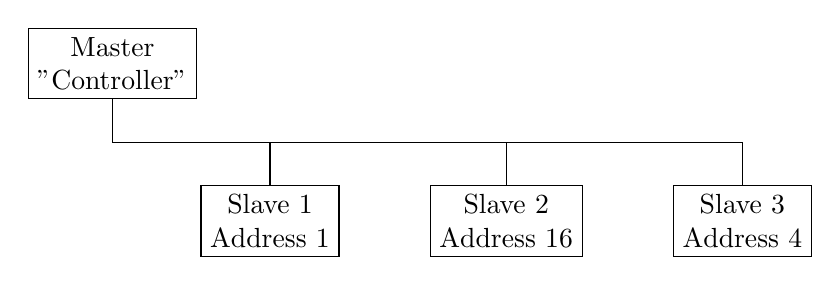
\begin{tikzpicture}
		\node[draw=black, align=center] (master) {Master\\''Controller''};
		\node[draw=black, align=center] (s1) at (2, -2) {Slave 1\\Address 1};
		\node[draw=black, align=center] (s2) at (5, -2) {Slave 2\\Address 16};
		\node[draw=black, align=center] (s3) at (8, -2) {Slave 3\\Address 4};

		\draw (master) -- (0, -1) -- (8, -1);
		\draw(s1) -- (2, -1);
		\draw(s2) -- (5, -1);
		\draw(s3) -- (8, -1);
	\end{tikzpicture}
\end{frame}

\section{A Linux I2C driver}
\begin{frame}[fragile]{A Linux I2C driver}{Header and compatible devices}
	\begin{lstlisting}
/* Required Header */
#include <linux/i2c.h>

/* Name all compatible devices*/
static struct i2c_device_id my_ids[] = {
	{"my_dev"},
	{} /* Empty element signalizes end of list */
};
MODULE_DEVICE_TABLE(i2c, my_ids);
	\end{lstlisting}
\end{frame}


\begin{frame}[fragile]{A Linux I2C driver}{Probe- and Remove functions}
	\begin{lstlisting}
/* function is called, when a compatible I2C device is added to the system */
static int my_probe(struct i2c_client *client)
{
	printk("Hello says I2C client with address: 0x%x\n", client->addr);
	return 0;
}

/* function is called, when a compatible I2C device is removed from the system */
static void my_remove(struct i2c_client *client)
{
	printk("Bye, bye, I2C\n");
}
	\end{lstlisting}
\end{frame}

\begin{frame}[fragile]{A Linux I2C driver}{Bundle driver struct}
	\begin{lstlisting}
/* Bundle compatbile devices, probe and remove functions and driver info into driver struct */
static struct i2c_driver my_driver = {
	.probe = my_probe,
	.remove = my_remove,
	.id_table = my_ids,
	.driver = {
		.name = "my-i2c-driver",
	}
};
/* Register driver at the OS */
module_i2c_driver(my_driver);
/* Information about the driver*/
MODULE_LICENSE("GPL");
MODULE_AUTHOR("Johannes Roith");
MODULE_DESCRIPTION("A Hello World I2C driver");
	\end{lstlisting}
\end{frame}

\section{Makefile for compiling the I2C driver}
\begin{frame}[fragile]{Makefile for compiling the I2C driver}
	\begin{lstlisting}[language=bash]
# Kernel Header Makefile compiles i2c_hello.c to i2c_hello.o file automatically
obj-m += i2c_hello.o

all:
	make -C /lib/modules/$(shell uname -r)/build M=$(PWD) modules

clean:
	make -C /lib/modules/$(shell uname -r)/build M=$(PWD) clean
	\end{lstlisting}
\end{frame}

\section{Module verwalten in einer Shell}
\begin{frame}[fragile]{Module verwalten in einer Shell}
	\begin{itemize}
		\item \lstinline|lsmod| lists all loaded modules
		\item \lstinline|dmesg| shows the kernel's log
		\item \lstinline|insmod <modulename>| load the module \lstinline|<modulename>| into the kernel
		\item \lstinline|rmmod <modulename>|  removes the module <\lstinline|modulename>| from the kernel
		\item \lstinline|modprobe <modulename>|  loads the module \lstinline|<modulename>| together with all its dependencies
		\item \lstinline|modinfo <modulename>|  shows the meta-data (author, licence, description, ...) of the module \lstinline|<modulename>|
	\end{itemize}
\end{frame}

\section{Adding I2C devices over sysfs}
\begin{frame}[fragile]{Adding I2C devices over sysfs}
	\begin{lstlisting}[language=bash]
# Change to I2C device folder
cd /sys/bus/i2c/devices/i2c-1

# Add I2C device mydev with address 0x12
echo "mydev 0x12" | sudo tee new_devices

# Removes I2C device with address 0x12
echo "0x12" | sudo tee delete_device
	\end{lstlisting}
\end{frame}

\begin{frame}{Exercise}
	\begin{itemize}	
		\item Implement the kernel module \lstinline|rgb_board| on the Raspberry Pi as follows:
			\begin{itemize}
				\item The name of the compatible device should be \lstinline|rgb_brd|
				\item The probe function should print out the I2C address of the device into the kernel's log
				\item Another kernel's log message should be written to the log when removing the device
			\end{itemize}
		\item Compile the kernel with the Makefile
		\item Load the module
		\item Check that the module is loaded
		\item Add a compatible I2C device
		\item Check the Kernel's log
		\item Remove the module
	\end{itemize}	
\end{frame}

\section{PCF8574 IO Expander}
\begin{frame}{PCF8574 IO Expander}
	\begin{itemize}
		\item Write access writes output values P0 - P7
		\item Read access reads current values P0 - P7
		\item Button connected to P0
		\item For input operation: Set Output to 1, Button pulls pin to GND. When reading a 1, the button is not pushed, when reading a 0 it is pushed
		\item Red LED connected to P1, green to P2, blue to P3
		\item Set output to 0: LED is On
		\item Set output to 1: LED is Off
	\end{itemize}

	\centering

	\begin{tabular}{lllllllll}
		Bit: & 0 & 1& 2& 3& 4& 5& 6& 7\\
		\hline
		Value for: & P0 & P1 & P2 & P3 & P4 & P5 &P6 & P7 \\
	\end{tabular}
\end{frame}

\section{Accessing the I2C bus}
\begin{frame}{Accessing the I2C bus}

\begin{block} {
                \lstinline|struct i2c_client *my_client|;
        }
		The \lstinline|struct i2c_client| is used, to manage an I2C device in the kernel. With the pointer \lstinline|my_client| we can access the device, e.g. for reading or writing data.
\end{block}

\begin{block} {
		\lstinline|s32 i2c_smbus_read_byte(struct i2c_client *my_client)|;
        }
	Reads a byte from the I2C device \lstinline|my_client|. If an error occurs, the function returns a negative error code, else the read byte.
\end{block}

\begin{block} {
		\lstinline|s32 i2c_smbus_write_byte(struct i2c_client *my_client, u8 value)|;
        }
	Writes the byte \lstinline|value| to the I2C device \lstinline|my_client|. If an error occurs, the function returns a negative error code, else 0.
\end{block}
\end{frame}

\begin{frame}{Exercise}
	\begin{itemize}	
		\item Light up the RGB LED in a color of your choice. You can do so, by writing to P1-P3 of the PCF8574 in the probe function of the driver.
		\item Turn off the RGB LED in the remove function
		\item Compile and test the module
		\item Additional task: Read the state of the button on P0 in the probe function and write it to the Kernel's log.
	\end{itemize}	
\end{frame}

\section{Creation of sysfs entries} 
\begin{frame}{Creation of sysfs entries}
	\begin{itemize}
		\item \textit{sysfs}: Virtual filesystem
		\item Display and management of \textit{Kernel Objects} (\lstinline|kobject|)
		\item Allows interaction with the driver
		\item \textit{Kernel Object}: Folder in \textit{sysfs}
		\item \textit{Kernel Object} can have attributes (represented as files) over which the driver can exchange data with user space.
		\item Procedure: Implement show and store functions, create attribute, create Kernel Object, link sysfs files with Kernel Object
	\end{itemize}
\end{frame}


\begin{frame}[fragile]{Show and store functions and attribute}
	\begin{lstlisting}
/* Required Header */
#include <linux/kobject.h>

static ssize_t mydev_show(struct kobject *kobj, struct kobj_attribute *attr, char *buffer)
{
	return sprintf(buffer, "Hello world!\n");
}

static ssize_t mydev_store(struct kobject *kobj, struct kobj_attribute *attr, const char *buffer, size_t count)
{
	printk("I got %s\n", buffer);
	return count;
}

static struct kobj_attribute mydev_attr = __ATTR(my_attr, 0660, mydev_show, mydev_store);
	\end{lstlisting}
\end{frame}

\begin{frame}[fragile]{Create kobject and link it with the attribute}
	\begin{lstlisting}
struct kobject * my_kobj */
/* in init or probe function */
int status;

my_kobj = kobject_create_and_add("my_kobj", my_kobj);
if (!my_kobj) {
	printk("Error creating kernel object\n");
	return -ENOMEM;
}

status = sysfs_create_file(my_kobj, &mydev_attr.attr);
if (status) {
	printk("Error creating /sys/my_kobj/my_attr\n");
	return status;
}
	\end{lstlisting}
\end{frame}

\begin{frame}[fragile]{Delete kobject and attribute}
	\begin{lstlisting}
/* in exit or remove function */
sysfs_remove_file(my_kobj, &mydev_attr.attr);
kobject_put(my_kobj);
	\end{lstlisting}
\end{frame}

\begin{frame}{Exercise}
	\begin{itemize}	
		\item Create the Kernel object \textit{rgb\_led}
		\item Create the attribute \textit{led} of the Kernel object \textit{rgb\_led}
		\item Implement the store function for this attribute, so you can control the RGB LED over it. By writing the string \lstinline|011| to the attribute, the red LED should be set t0 0, the green LED to 1 and the blue LED to 1.
		\item Additional Task: Create a second attribute \textit{button} of the Kernel Object \textit{rgb\_led}. Implement a show function to read out the current state of the button.
	\end{itemize}	
\end{frame}

\section{A true Hello World Kernel Module}
\begin{frame}[fragile]{A true Hello World Kernel Module}
	\begin{lstlisting}
#include <linux/module.h>
#include <linux/init.h>
int __init my_init(void)
{
	printk("hello_kernel - Module was loaded.\n");
	return 0;
}
void __exit my_exit(void)
{
	printk("hello_kernel - Module was removed\n");
}
MODULE_LICENSE("GPL");
MODULE_AUTHOR("Johannes Roith");
MODULE_DESCRIPTION("A simple hello world LKM");
module_init(my_init);
module_exit(my_exit);
	\end{lstlisting}
\end{frame}

\section{The macro module\_i2c\_driver}
\begin{frame}[fragile]{The macro module\_i2c\_driver}
	The macro \lstinline|module_i2c_driver(my_driver)| creates the following code:

	\begin{lstlisting}
static int i2c_driver_init(void)
{
	return i2c_add_driver(&my_driver);
}
module_init(i2c_driver_init);

static void i2c_driver_exit(void)
{
	i2c_del_driver(&my_driver);
}
module_exit(i2c_driver_exit);
	\end{lstlisting}
\end{frame}

\end{document}
